\documentclass[a4paper,italian,10pt,openany]{book}
\usepackage[english]{babel}
\usepackage{lipsum}
\usepackage{longtable}
\usepackage{graphicx}
\usepackage{makeidx}
\usepackage{hyperref}
\usepackage[document]{ragged2e}
\usepackage{fancyhdr}
\usepackage{geometry}
\geometry{a4paper, top=3cm, bottom=3cm, left=1.5cm, right=1.5cm, heightrounded, bindingoffset=5mm}


\begin{document}
\clearpage
\newcommand\nbvspace[1][3]{\vspace*{\stretch{#1}}}
% allow some slack to avoid under/overfull boxes
\newcommand\nbstretchyspace{\spaceskip0.5em plus 0.25em minus 0.25em}
\begin{titlepage}
\begin{center}
\tt
\nbvspace[0.03]
\begin{tabular}[c]{@{}c@{}}\vspace{0.1cm}\textbf{\LARGE{UNIVERSITA' DEGLI STUDI DI NAPOLI FEDERICO II}}\\\vspace{0.1cm}\Large{SCUOLA POLITECNICA E DELLE SCIENZE DI BASE}\\\large{DIPARTIMENTO DI INGEGNERIA ELETTRICA E TECNOLOGIE DELL'INFORMAZIONE}\end{tabular}


\includegraphics[width=4cm]{LOGO}
\nbvspace[0.1]
\begin{tabular}[c]{@{}c@{}}\vspace{0.1cm}\Large{CORSO DI LAUREA IN INFORMATICA}\\\vspace{0.1cm}\Large{INSEGNAMENTI DI BASI DI DATI E PROGRAMMAZIONE AD OGGETTI}\\\Large{ANNO ACCADEMICO 2022/2023}\end{tabular}
\rm
\begin{tabular}[c]{@{}c@{}}\huge{\textbf{Progettazione e sviluppo di una base di dati}}\\\huge{\textbf{relazionale per la descrizione e la}}\\\huge{\textbf{memorizzazione di conferenze scientifiche}}\end{tabular}
\end{center}
\begin{longtable}[c]{llr}
\textit{Autori:}                                                                                                                   &  & \textit{Docenti:}                                                                        \\
\endhead
%
\begin{tabular}[c]{@{}l@{}}ALESSANDRO GRIECO\\      Matricola N86/4241\\      alessandro.grieco2@studenti.unina.it\end{tabular}    &  & \begin{tabular}[c]{@{}r@{}}Prof. Sergio Di Martino \end{tabular} \\
\begin{tabular}[c]{@{}l@{}}GIANFRANCO DUMINUCO\\      Matricola N86/4061\\      gianfranco.duminuco@studenti.unina.it\end{tabular} &  & \multicolumn{1}{l}{}                                                                    
\end{longtable}                  
\end{titlepage}
\tableofcontents
    \chapter{Introduzione}
    \section{Descrizione introduttiva}
	Si progetterà un programma applicativo alla gestione di Conferenze Scientifiche con lo scopo mirato all'accesso mediante un interfaccia grafica che permetterà all'Utente di manipolare il complesso organizzativo delle conferenze. Il Sistema garantisce tutte le funzionalità indicate nella traccia e altre funzionalità secondarie non palesate nella traccia ma aggiunte per una maggiore usabilità. Il programma applicativo, ignora come le informazioni esterne vengono reperite: fa un utilizzo esclusivo di informazioni presenti nella base di dati.
	\section{Traccia}
	Si sviluppi un sistema informativo, composto da una base di dati relazionale e da un applicativo Java dotato di GUI (Swing o JavaFX), per la gestione di conferenze scientifiche. Ogni conferenza ha una data di inizio e di fine, una collocazione (sede, indirizzo), uno o più enti che la organizzano, degli sponsor (che coprono in parte le spese), una descrizione, ed un gruppo di organizzatori, che può essere distinto in comitato scientifico e comitato  locale  (che  si  occupa  cioè  della  logistica).  Di  ognuno  degli  organizzatori,  così  come  di  tutti  i partecipanti si riportano titolo, nome, cognome, email ed istituzione di afferenza. Ogni conferenza può avere una o più sessioni, anche in parallelo fra loro. Ogni sessione ha una locazione all'interno della sede. Per ogni sessione c'è un programma, che prevede la presenza di un coordinatore (chair) che gestisce la sessione, ed eventualmente di un keynote speaker (un partecipante di particolare rilievo invitato dagli organizzatori). Ogni sessione  avrà  quindi  una  successione  di  interventi,  ad  orari  predefiniti  e  di  specifici  partecipanti.  Per  ogni intervento si conserva un abstract (un breve testo in cui viene spiegato il contenuto del lavoro presentato). Si deve poter considerare la presenza di spazi di intervallo (coffee breaks, pranzo) ma anche la presenza di eventi sociali (cene, gite, etc). L’interfaccia deve prevedere la possibilità di aggiunta, cancellazione e modifica di una conferenza. Inoltre l’utente deve avere la possibilità di poter visualizzare tutte le conferenze che si terranno  in  una  specifica  data  o  intervallo  di  tempo,  eventualmente  filtrando  anche  per  sede.  Per  ogni conferenza l’utente deve poter visualizzare la scaletta degli interventi (eventualmente ordinatianche  per giorno) compresa di intervalli (coffe break, pranzo, cene, gite etc.); e per ogni intervallo l’utente deve avere la possibilità di poternevisualizzare la descrizione.Infine,si vorrebbe un riepilogo, su base mensilee annuale, sullapercentualedelleistituzioni  di  afferenza a  cui  appartengono  gli  speakerche  hanno  sostenutounaconferenzain quel mese/anno.
	\section{Individuazione delle classi}
	\begin{enumerate}
	\item \textbf{Conferenza}: ;
	\item \textbf{Sponsor}: classe che permette la memorizzazione di Aziende che vengono sponsorizzate;
	\item \textbf{Sede}: classe che mira a gestire il luogo geografico della Conferenza;
	\item \textbf{Locazione}: classe per la visualizzazione della struttura interna alla Sede ove si terrà la Sessione;
	\item \textbf{Programma}: classe intermediaria tra la Conferenza e la organizzazione tempistica tra Sessione, intervallo ed evento sociale. Utile a creare coerenza sia con le date proposte dalla conferenza (dataInizio e dataFine) e sia con gli orari tra Sessione, Intervallo ed Evento Sociale;
	\item \textbf{Sessione}: classe per la gestione delle sessioni in un programma. Garantisce inoltre anche la possibile presenza di partecipanti nelle vesti keynote speaker, o di organizzatori scientifici nelle vesti di chair;
	\item \textbf{Evento Sociale}: classe per la gestione degli eventi sociali in un programma;
	\item \textbf{Intervallo}: classe per la gestione degli intervalli in un programma;
	\item \textbf{Intervento}: classe che gestisce la durata degli interventi proposti in una sessione dai partecipanti;
	\item \textbf{Partecipante}: classe per la visualizzazione di informazioni riguardanti gli spettatori della Sessione;
	\item \textbf{Ente}: classe responsabile degli enti che amministrano una conferenza scientifica, definendo così gli organizzatori scientifici e locali;
	\item \textbf{Organizzatore Locale}: classe che memorizza informazioni riguardanti un organizzatore locale (o tecnico);
	\item \textbf{Organizzatore Scientifico}: classe che memorizza informazioni riguardanti un organizzatore scientifico, e gestisce la possibilità di definire un chair di una Sessione;
	\item \textbf{Pubblicità}: classe di associazione tra Sponsor e Conferenza per la visualizzazione della spesa pubblicitaria che copre parzialmente il costo della conferenza;
	\item \textbf{Utente}: generalizzazione di tipo "Organizzatore Locale" o "Organizzatore Scientifico".
	\end{enumerate}
	\section{Individuazioni delle Responsabilità}
	Nell'individuazione delle responsabilità delle classi, andremo a attribuire un \textbf{requisito funzionale} richiesto al sistema.
\begin{itemize}
\item Un utente avrà la possibilità di:
	\begin{itemize}
	\item[-] Modificare una conferenza esistente.
	\item[-] Cancellare una conferenza esistente.
	\item[-] Aggiungere una conferenza
	\end{itemize}
\item Un utente non loggato avrà la possibilità di:
	\begin{itemize}
	\item[-] Ricerca di conferenze per i seguenti filtri : \textit{data},  \textit{intervallo di tempo}, \textit{sede}.
	\item[-] Visualizzazione delle sedute compresi di intervallo sessione ed eventi sociali.
	\item[-] Visualizzazione delle descrizione di ogni sessione.
	\end{itemize}
	\item Una conferenza avrà la possibilità di:
	\begin{itemize}
	\item[-]Gestire operazioni sui programmi (come eliminazione, aggiunta e impostazioni alle varie date della conferenza)
	\end{itemize}
	\item Un Ente avrà la responsabilità di amministrare la conferenza, il quanto definirne gli organizzatori locali e scientifici
	\item Un organizzatore scientifico avrà la possibilità di definirsi chair di una conferenza.
\end{itemize}
\let\cleardoublepage\clearpage
	\chapter{CRC CARDS E DIAGRAMMI}
	A seguire, verranno presentate le \textbf{Class Responsibility Collaboration}. Per ogni classe identificata , verrà posto il nome della classe sulla scheda (Card). Accompagnate ad esse sarà illustrato il class diagram riferitosi. Ecco un CARD illustrativa da campione per la lettura delle CRC CARDS:
	\begin{figure}[h!]
	\centering
	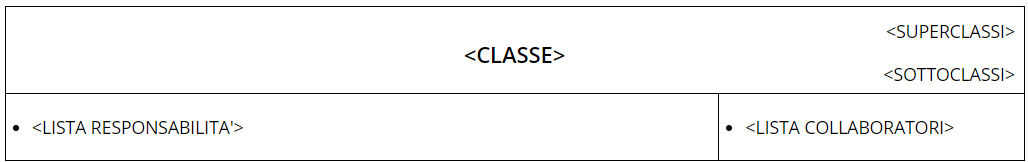
\includegraphics[width=16cm]{crc_cardsEx}
	\end{figure}
	%%--da riempire
	\newpage
	%%--class diagram MODEL
	\section{CRC Cards - MODEL}
	\begin{figure}[h!]
	\centering
	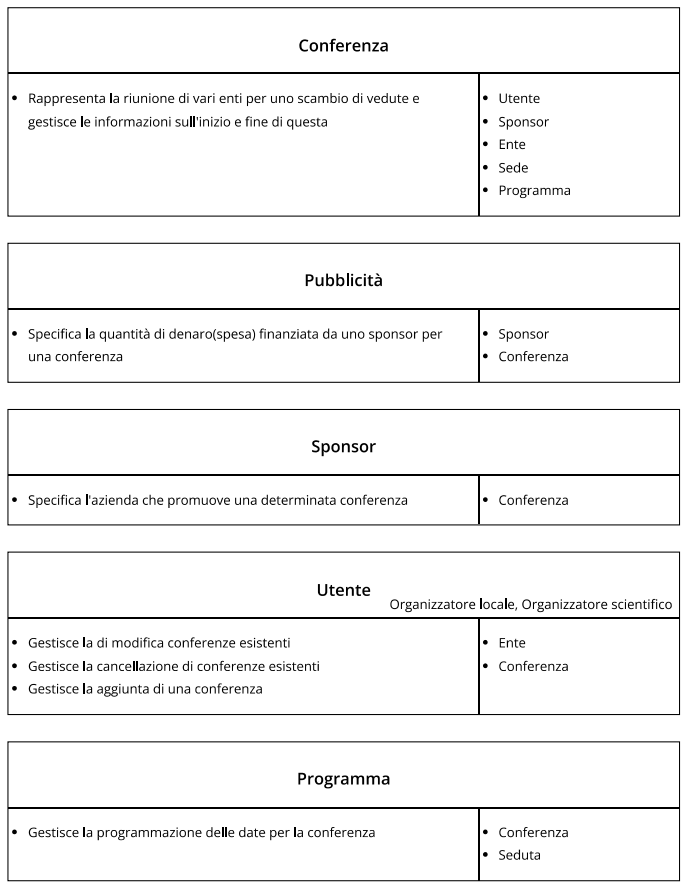
\includegraphics[width=15.8cm]{crc_cards1}
	\end{figure}
	\begin{figure}[h!]
	\centering
	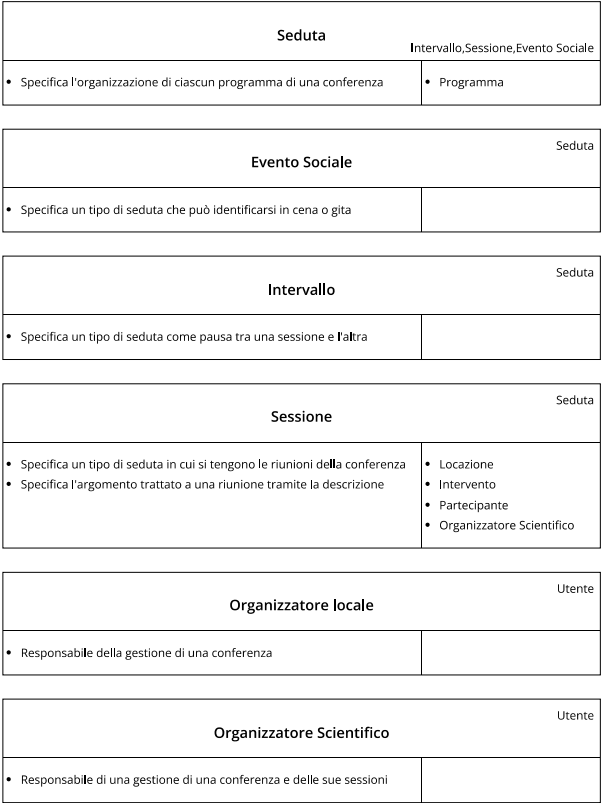
\includegraphics[width=17cm]{crc_cards2}
	\end{figure}
	\begin{figure}[h!]
	\centering
	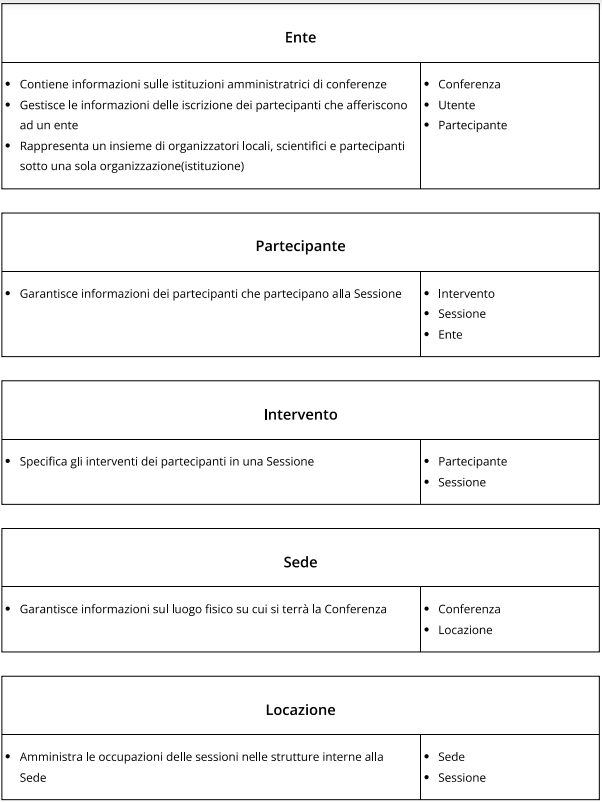
\includegraphics[width=17cm]{crc_cards3}
	\end{figure}
	\newpage
	\subsection{Class diagram - MODEL}
	\vspace{2cm}
	\begin{figure}[h!]
	\centering
	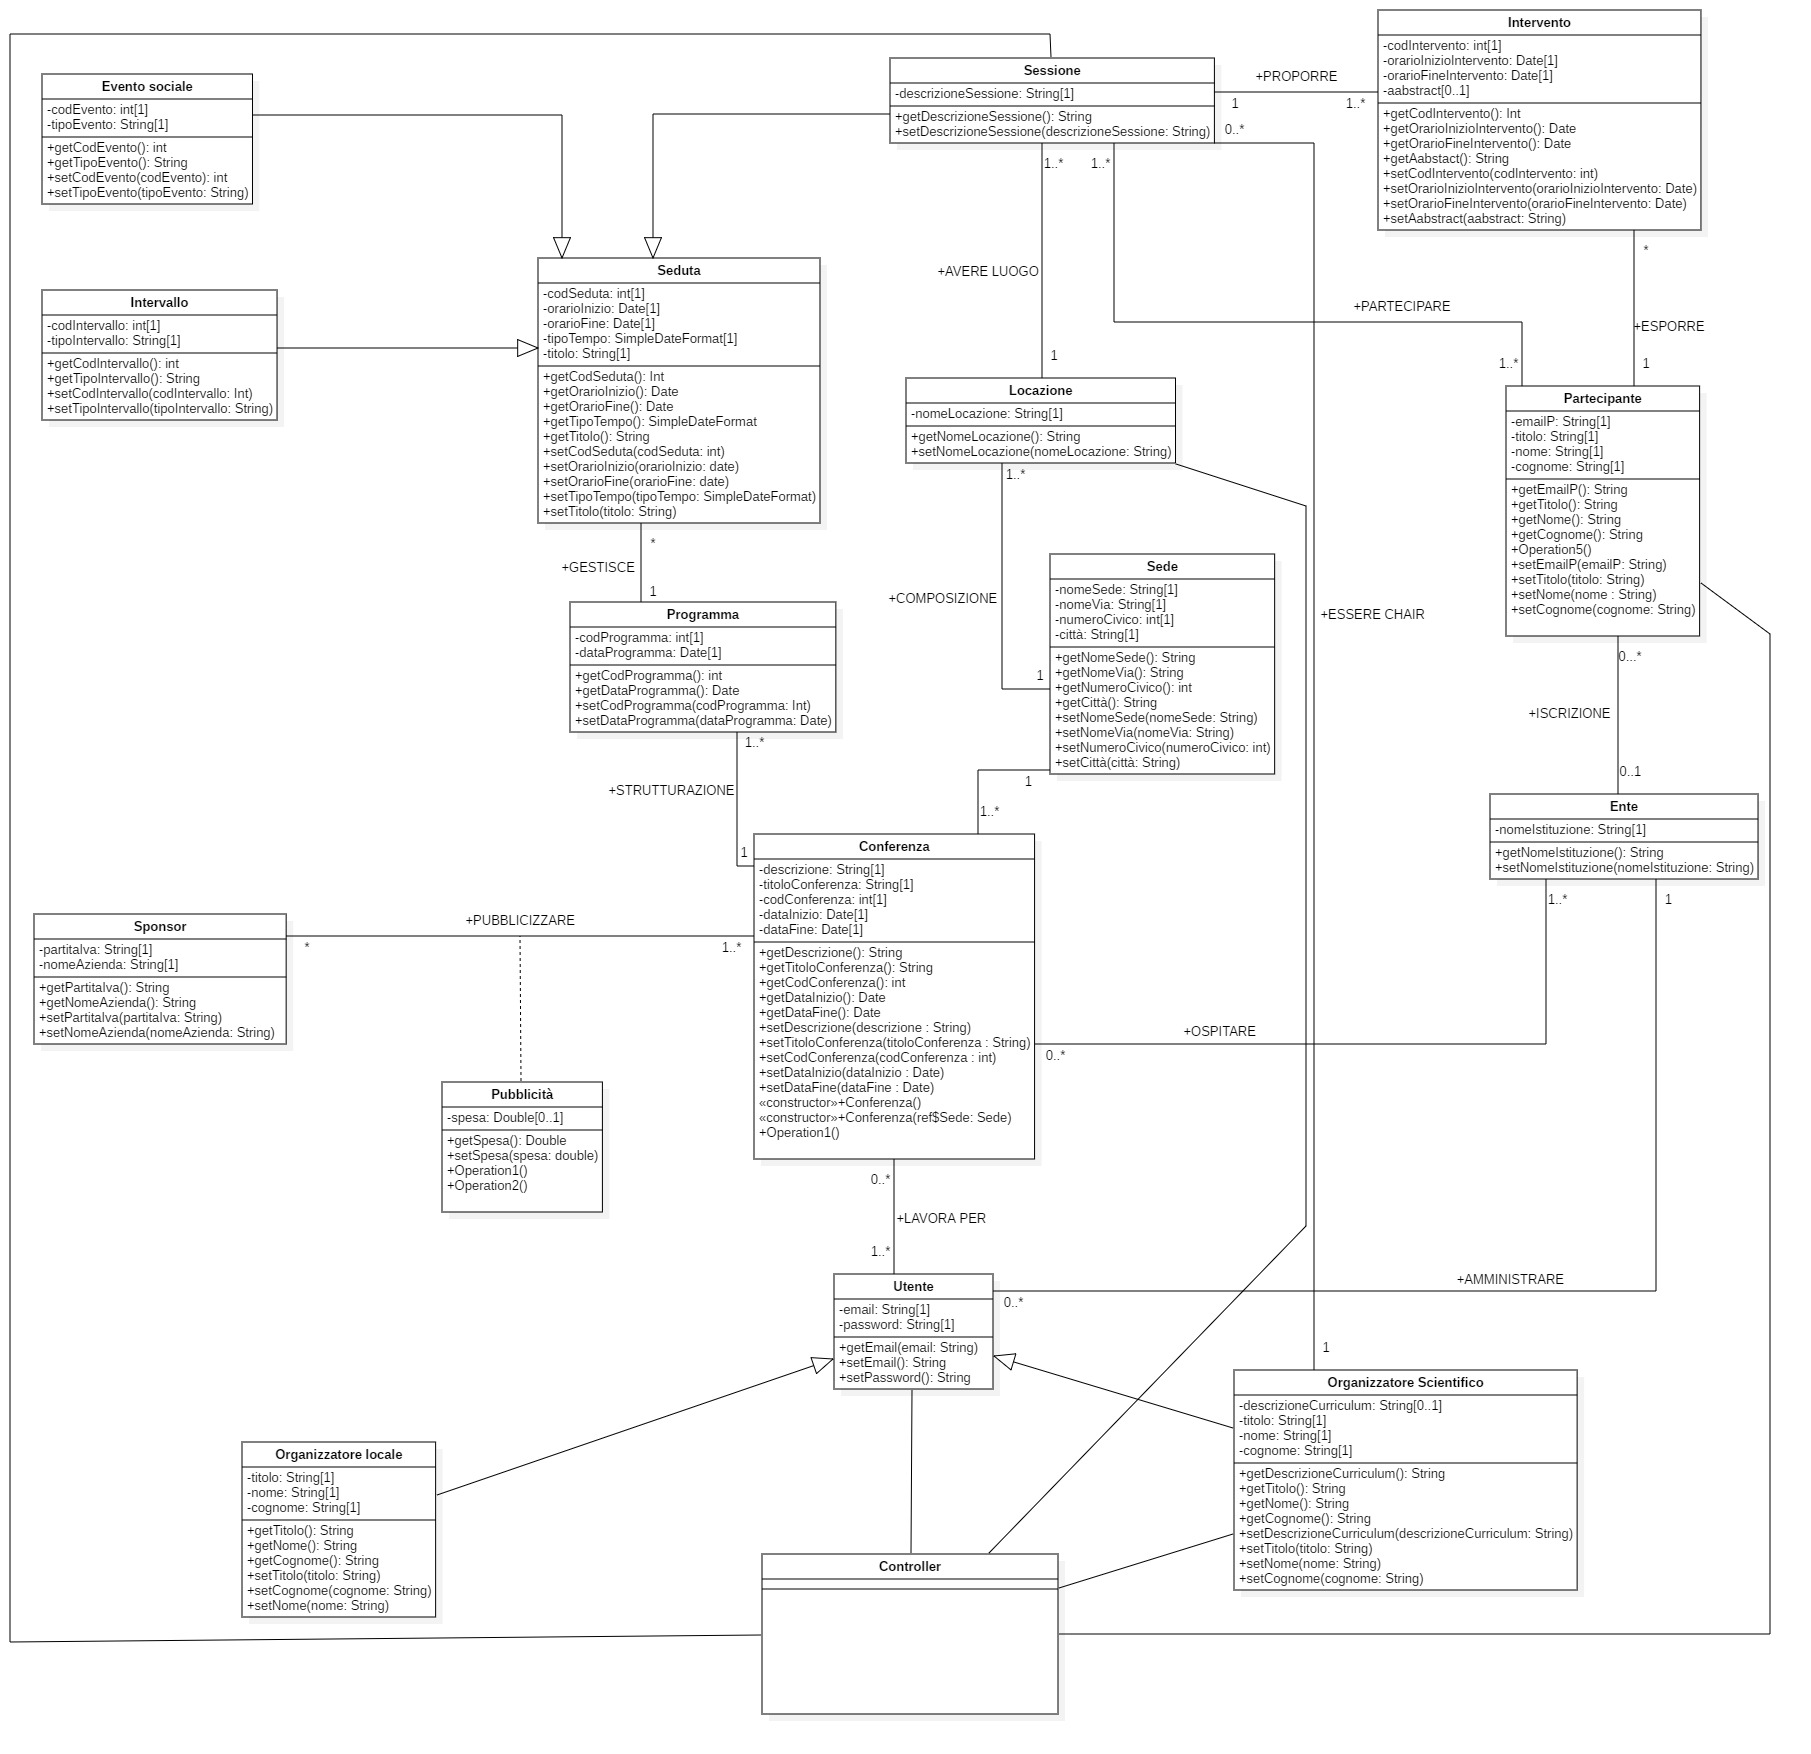
\includegraphics[width=18cm]{ClassDiagram MODEL}
	\end{figure}
	\newpage
	%%---class diagram GUI

\section{CRC Cards - GUI}
\begin{figure}[h!]
\centering
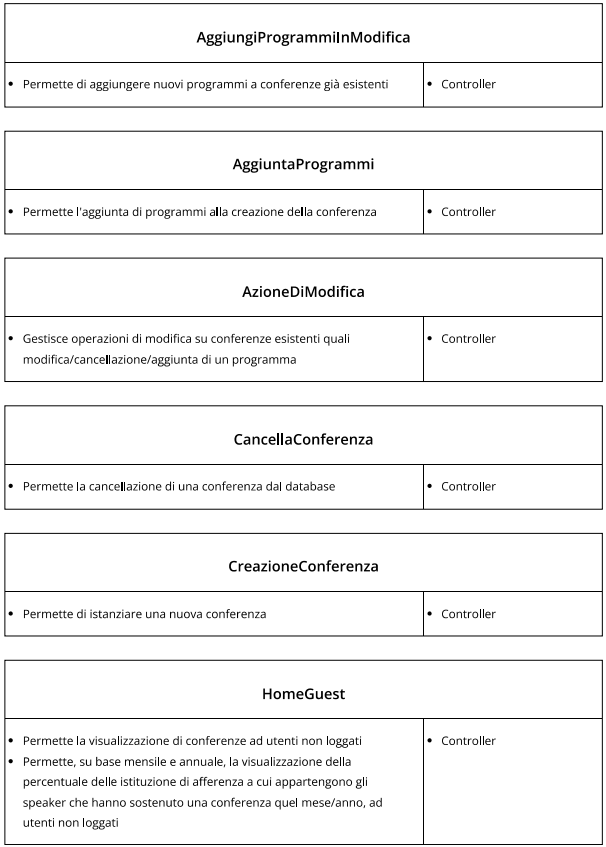
\includegraphics[width=15cm]{crc_card_gui1}
\end{figure}
\begin{figure}[h!]
\centering
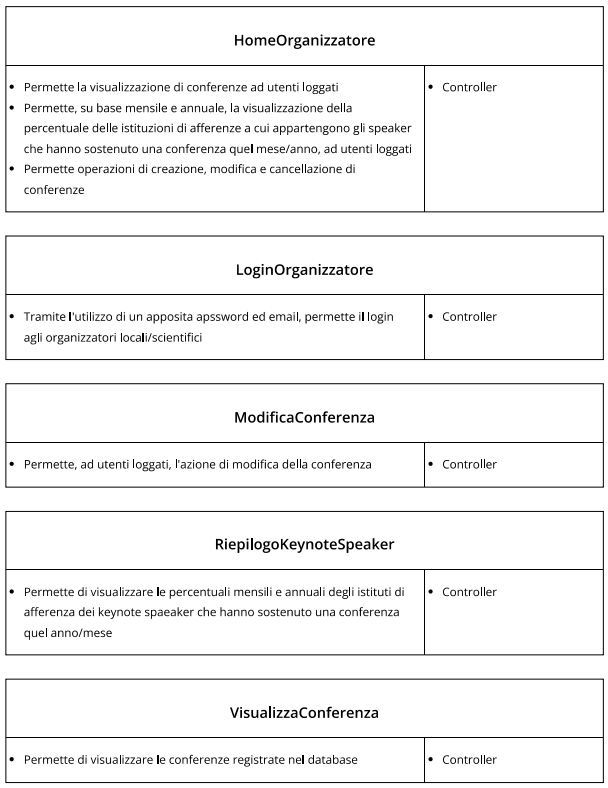
\includegraphics[width=13cm]{crc_card_gui2}
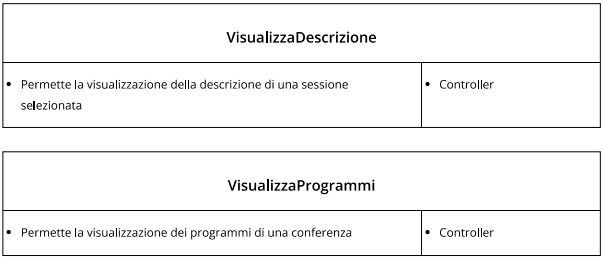
\includegraphics[width=13cm]{crc_card_gui3}
\end{figure}
\subsection{Class diagram - GUI}
\vspace{4cm}
\begin{figure}[h!]
\centering
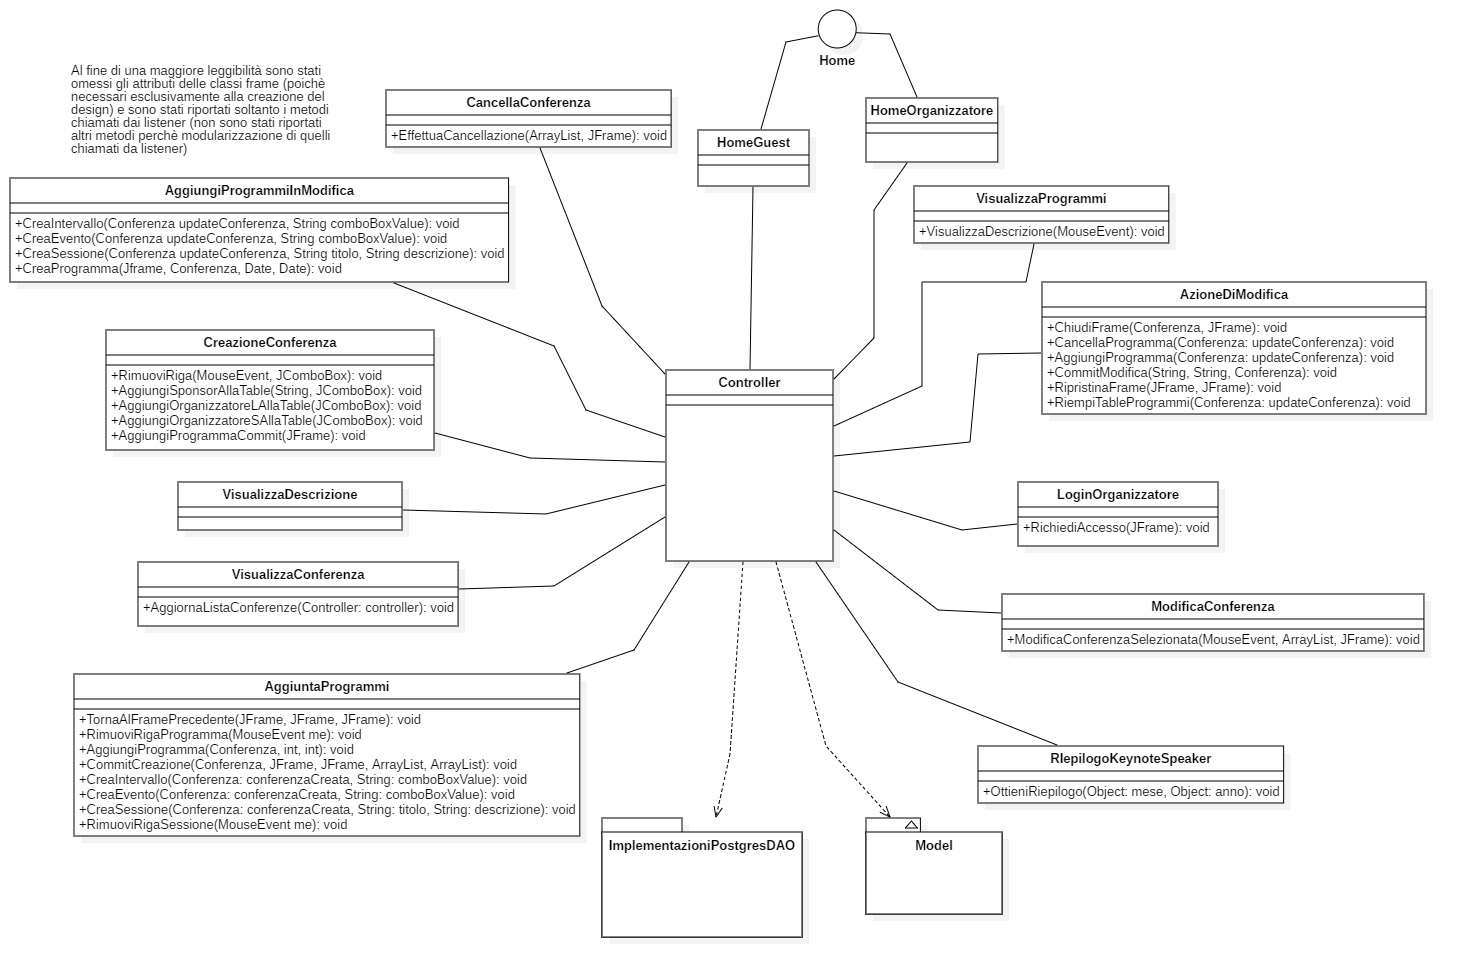
\includegraphics[width=18cm]{ClassDiagram GUI}
\end{figure}
\newpage
\section{CRC Cards - ImplementazionePostgresDAO}
\begin{figure}[h!]
\centering
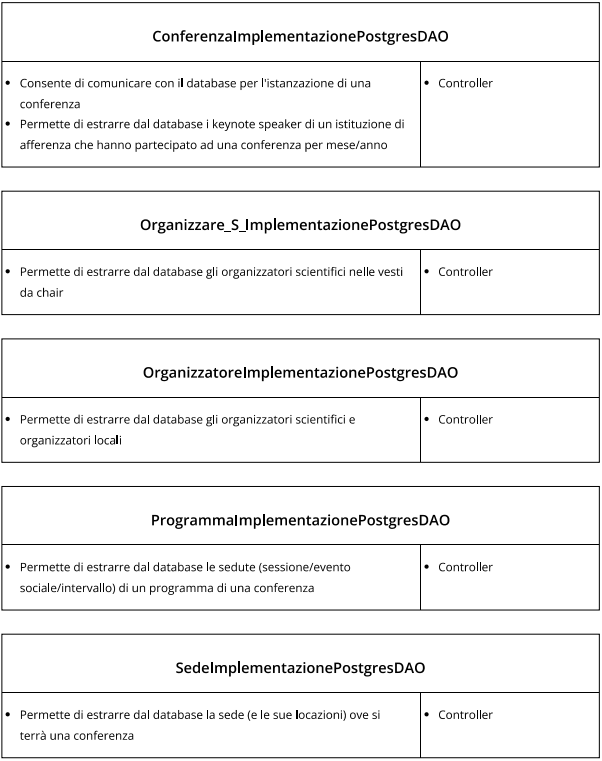
\includegraphics[width=11cm]{crc_card_dao1}
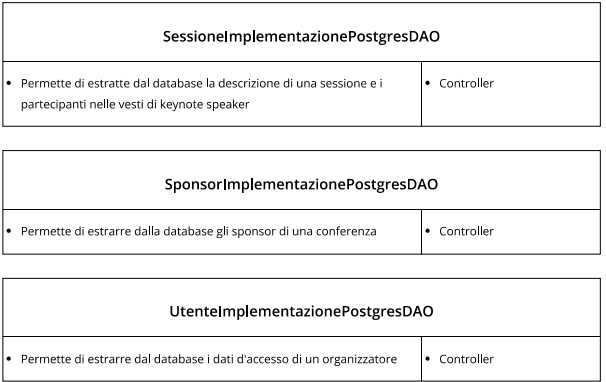
\includegraphics[width=11cm]{crc_card_dao2}
\end{figure}
\begin{figure}[h!]
\centering
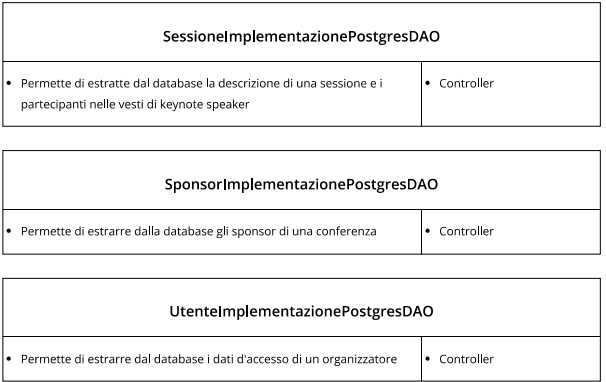
\includegraphics[width=13cm]{crc_card_dao2}
\end{figure}
\newpage
\subsection{Class diagram - ImplementazionePostgresDAO}
\vspace{3cm}
\begin{figure}[h!]
\centering
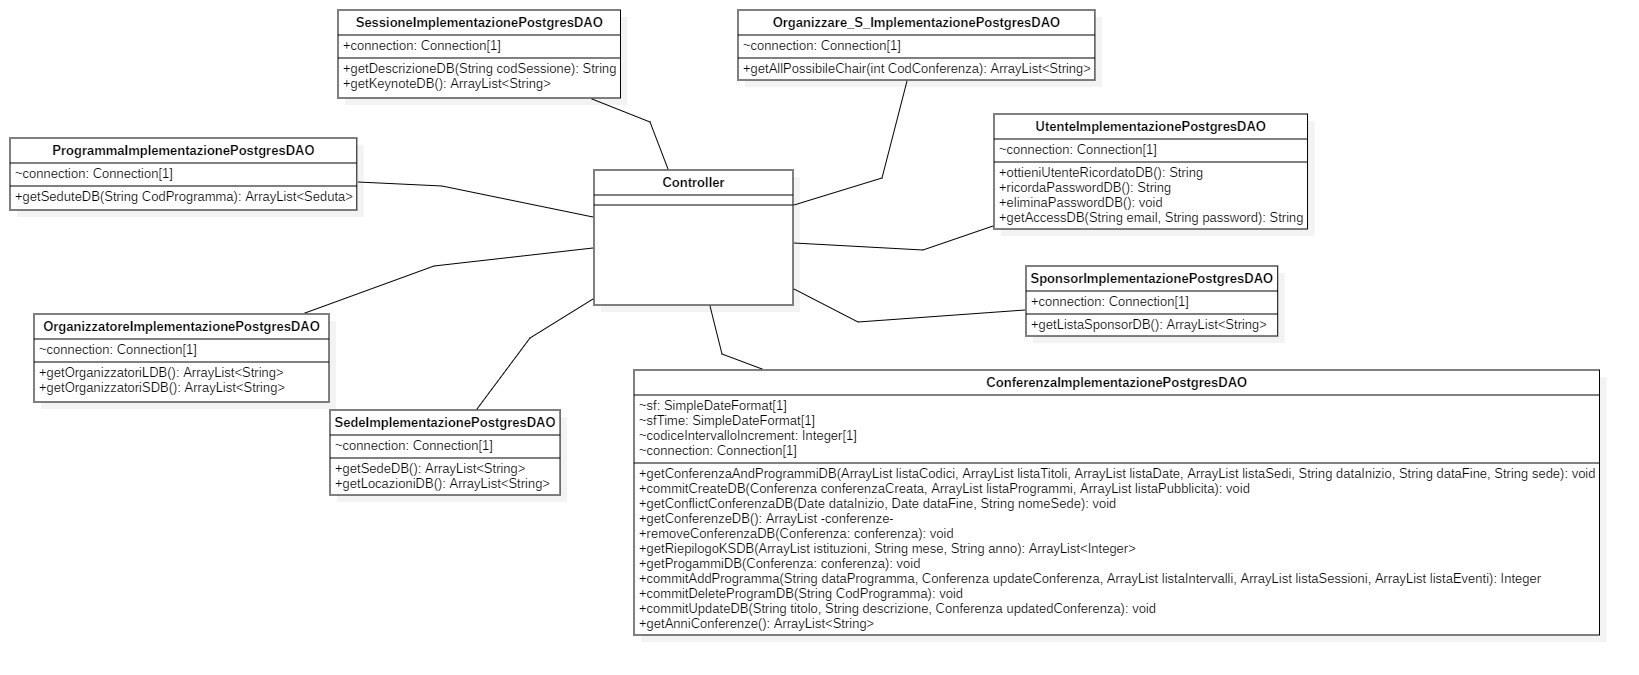
\includegraphics[width=19cm]{ClassDiagram DAO}
\end{figure}
\newpage
\section{Class diagram Controller}
\vspace{5cm}
\begin{figure}[h!]
\centering
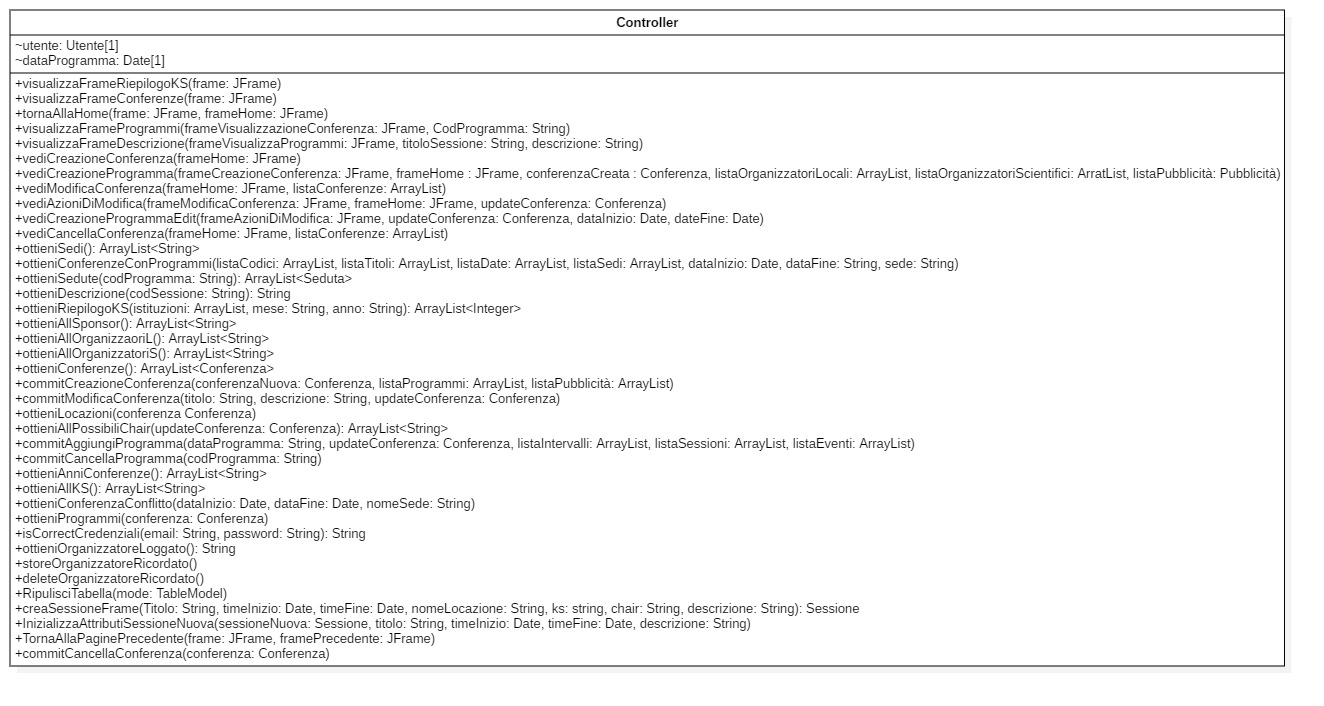
\includegraphics[width=16cm]{ClassDiagram CONTROLLER}
\end{figure}
\chapter{Sequence Diagram}
\vspace{4cm}
\section{Scelta della Home}
\begin{figure}[h!]
\centering
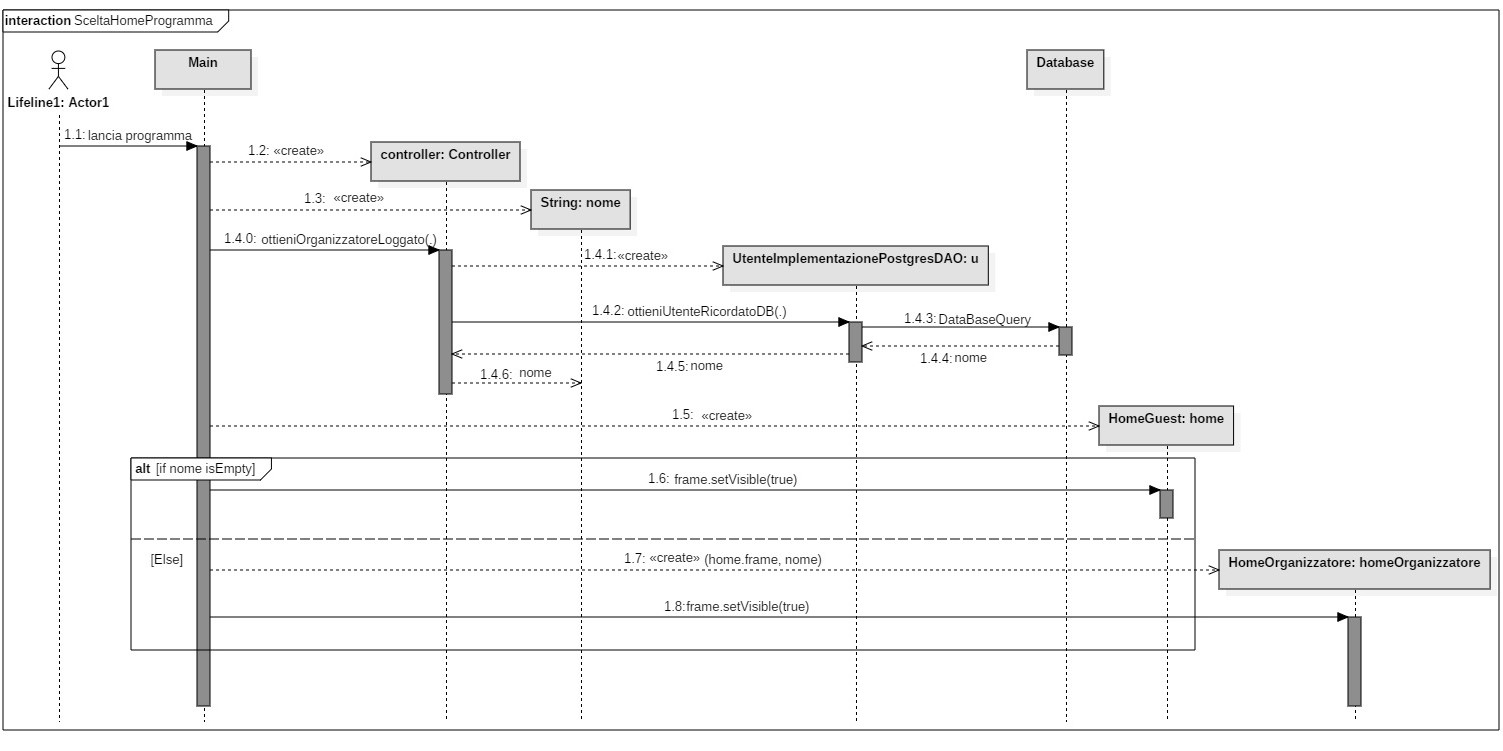
\includegraphics[width=18cm]{SD1}
\end{figure}
\newpage
\section{Accesso organizzatore}
\vspace{4cm}
\begin{figure}[h!]
\centering
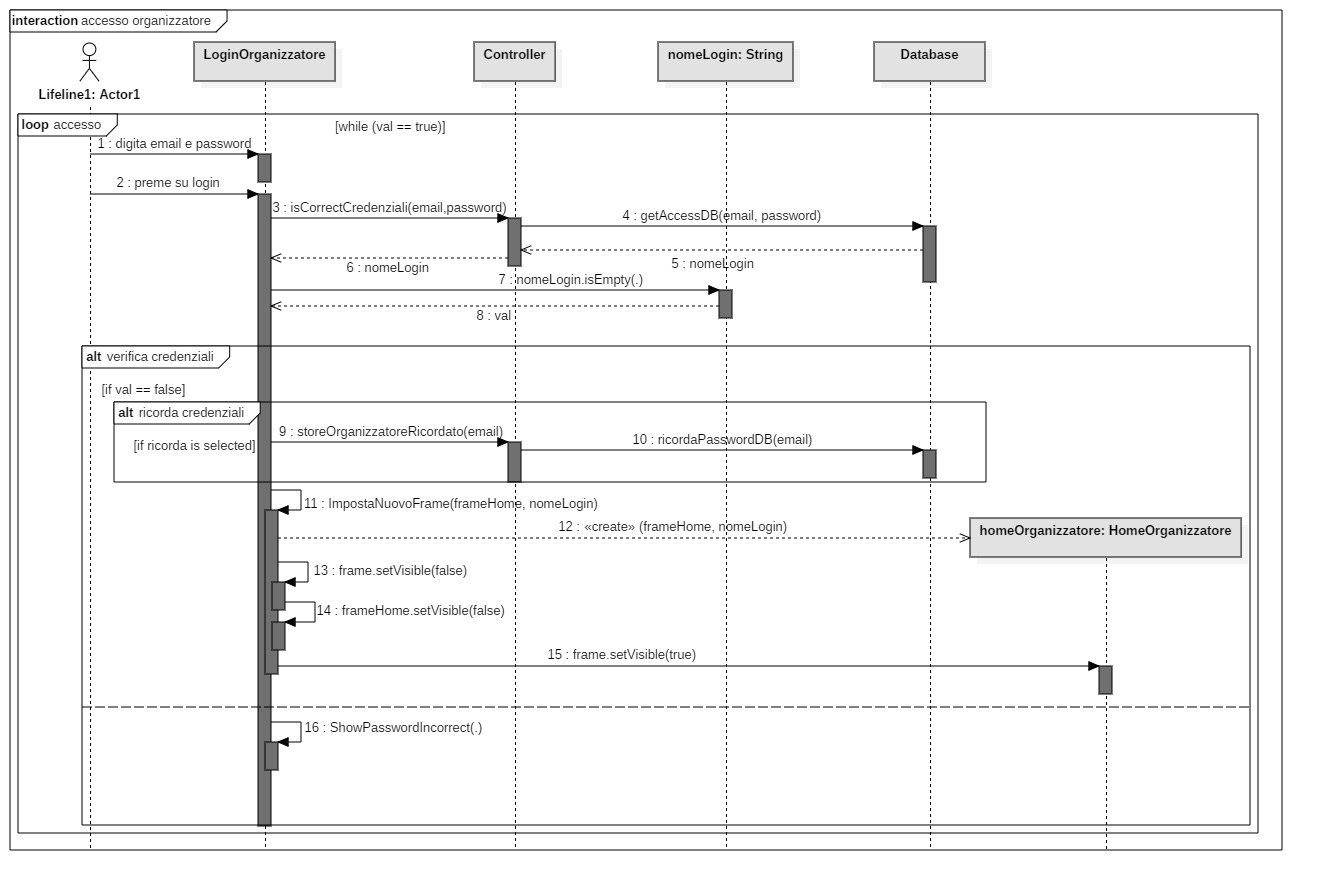
\includegraphics[width=18cm]{SD2}
\end{figure}
\newpage
\section{Struttura mock up}
\vspace{.5cm}
\begin{figure}[h!]
\centering
\includegraphics[width=14.5cm]{mockup}
\end{figure}
\end{document}